\section{Videoplayer}
\subsection{Ziel}
In einem ersten Schritt, vor der Realisierung des Fahrsimulator, wird ein Videoplayer ralisiert. Das Ziel dabei ist der Aufbau und Test der Anbindung der Eingabehardware an unser Programm. Bei der Betätigung des Gaspedals im Cockpit soll das aufgenommene Video schneller abgespielt werden. Bei der Betätigung des Bremspedals dementsprechend langsamer. Der Videoplayer soll so aufgebaut werden, dass Komponenten davon auch im Fahrsimulator wiederverwendet werden können. Die ETH Zürich besitzt bereits Videos, die sich gut dafür eigenen. Um Experimente mit diesen Videos durchführen zu können, müssen Eingaben, die der Proband im Cockpit mach, mit der aktuellen Position des Videos abgespeichert werden. Dies dient zur späteren Auswertung der Experimente.
\\
\subsection{Systembeschreibung}

Um einzelne Komponenten des Videoplayer wiederverwenden zu können, wird das System möglichst gleich wie das des Fahrsimulators aufgebaut. Dieser Aufbau wird anhand der Abbildung \ref{Systembeschreibung Videoplayer} illustriert. Blau markiert sind neu entwickelte Komponenten des Videoplayers. Die Eingaben im Cockpit werden von einem LabVIEW-Programm über eine USB-Schnittstelle eingelesen. Die eingelesenen Parameter werden, zusammen mit einem Timestamp, von LabVIEW in ein UDP-Paket verpackt und über einen UDP-Socket gesendet. Das Paket wird von einem UDP-Listener empfangen und gelesen. Dieser speichert die Daten ab und hält sie für das Hauptprogramm bereit. Das Hauptprogramm (Main Application) liest die gespeicherten Parameter aus und interpretiert diese. Der \gls{mplayer}, der für das Abspielen der Videos verwendet wird, lässt sich durch Konsoleneingaben über die Standard-In-Pipe steuern. So wird ihm vom Videoplayer mitgeteilt, wie schnell das aktuelle Video abgespielt werden soll.  Über die Standard-Out-Pipe gibt MPlayer die aktuelle Abspielposition zurück. Das Hauptprogramm wertet diese aus, ergänzt sie mit Benutzereingaben und leitet sie über den UDP-Listener an LabVIEW weiter. Dort werden die Daten über  einen zweiten UDP-Socket empfangen und in ein Log-File gespeichert, damit sie für Auswertungen zur Verfügung stehen.
\newpage

% Bild für Systembeschreibung des Video Players
\begin{figure}[H]
\centering 
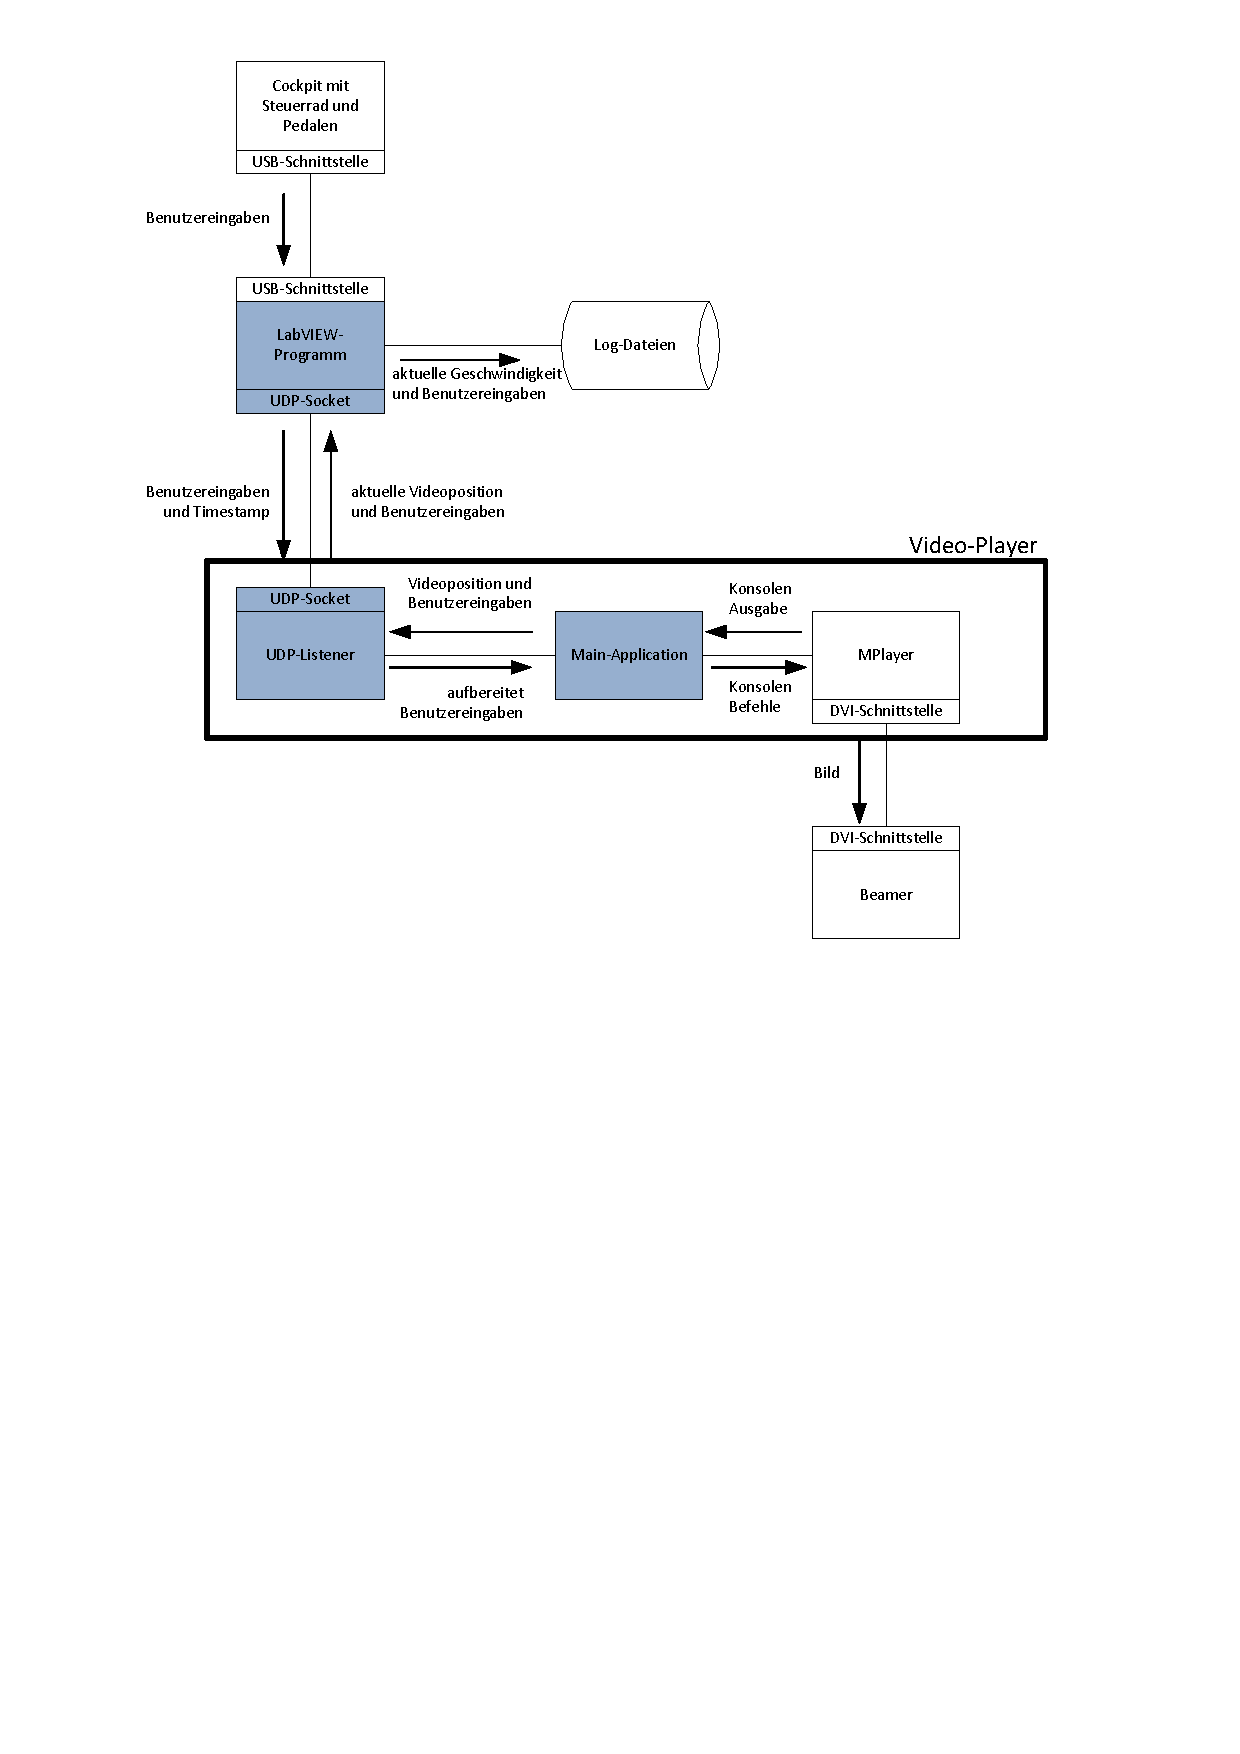
\includegraphics[width=0.8\linewidth]{src/Systembeschreibung_VideoPlayer.pdf}
\caption{Systembeschreibung Videoplayer} % Titel der Grafik
\label{Systembeschreibung Videoplayer} % Labelname
\end{figure}

\subsection{Realisierung}
Bei der Realisierung des Videoplayers wird der Fokus vorallem auf die Entwicklung der LabVIEW-Schnittstelle mit unserem Programm gelegt. Darum wird dieser Schritt der Realisierung nachfolgend ausführlich erklährt. Diese Schnittstelle wird auch für den Fahrsimulator selbst verwendet. Die Realisierung des Videoplayers wird ebenfalls erläutert.

\subsubsection{LabVIEW-Schnittstelle}
\label{labview_schnittstelle}
Die Realisierung der LabVIEW Schnittstelle wird in zwei Teile unterteilt. Der erste Teil dient dazu die Eingaben, die im Cockpit gemacht werden, einzulesen und an den UDP-Listener zu senden. Der zweite Teil befasst sich mit dem Empfangen von Daten, die vom UDP-Listener gesendet werden und dessen speicherung in ein LogFile.

\newpage 

% LabVIEW Screenshot um Daten zu senden
\begin{figure}[H]
\centering 
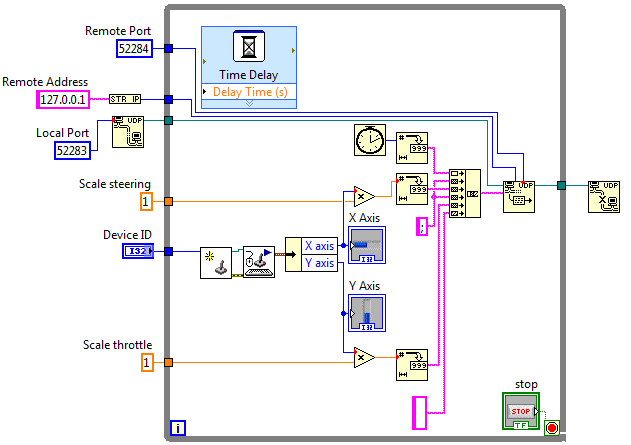
\includegraphics[width=1\linewidth]{src/labview_screenshot_videoplayer_daten_senden.png}
\caption{LabVIEW: Daten senden} % Titel der Grafik
\label{labview_screenshot_videoplayer_daten_senden} % Labelname
\end{figure}
Die Abbildung \ref{labview_screenshot_videoplayer_daten_senden} illustriert den Aufbau des LabVIEW-Programms um die Cockpitparameter zu lesen und über einen UDP-Socket zu senden.\\
Die \textit{Remot Address} gibt an für an wen das UDP-Packet gesendet. Da sich der UPD-Listener zur Zeit noch auf dem selben Rechner wie dieses Programm befindet, wählen wir hierfür die localhost-Adresse. Für den \textit{Remote Port} wählen wir einen freien Port, hier 52284. Zusammen mit dem \textit{Local Port}, der uns eine Verbindungs-ID generiert ist unsere Konfiguration für den UDP-Socket vollständig. Um die Komponenten im Cockpit ansprechen zu können muss lediglich die Richtige \textit{Device ID} gewählt werden. Die anderen Komponenten, die sich in der grauenn Box befinden werden in einer Schleife 100 mal pro Sekunde ausgeführt. Dieser Wert wird im \textit{Time Delay} Element konfiguriert. \\
Aus dem Cockpit werden die Werte der x- und y-Achse ausgelesen. Auf der y-Achse werden die beiden Pedalen, Gas- und Bremspedal, abgebildet. Ein negativer Wert auf der y-Achse quantiviziert hierbei das Drücken des Gaspedals, ein positiver Wert das Drücken des Bremspedals. Die Intensität beider Pedalen wird im Positiven durch 32767 und im Negativen durch 32768 ganzzahlige Werte quantiviziert. Ein voll gedrücktes Gaspedal entspricht also dem Wert -32768 auf der y-Achse und ein voll gedrücktes Bremspedal entspricht dem Wert 32767. Die x-Achse quantifiziert analog dazu den Einschlagswinkel des Steuerrades. Hierbei ist, wenn das Steuerrad sich in der neutralen Position befindet, der x-Wert null. Komplett nach rechts eingeschlagen beträgt der x-Wert 32767 und -32768 bei einem Einschlag nach links. Der x-Wert wird ebenfalls ausgelesen ist aber im Video-Player nicht relevant. Die beiden Werte werden je mit einem separatem Faktor multipliziert, um eventuell eine Anpassung derjenigen vorzunehmen. Danach werden sie zusammen mit aktuellen Timestamp durch Semikolons voneinander getrennt, in das UDP-Paket gepackt und dann versendet. Nach Verlassen der Schleife wird der UDP-Socket wieder geschlossen.

Die Abbildung \ref{labview_screenshot_videoplayer_daten_empfangen} illustriert den Aufbau des LabVIEW-Programms um die Daten zu empfangen und in ein Log-File zu speichern.\\
Es wird ein UDP-Socket geöffnet um ankommende Pakete zu empfangen. Der \textit{Local port} mit dem UDP-Verbindungskästchen gibt wieder eine Connection-ID die für das öffnen des UPD-Portes benötigt wird. Durch die Angaben von \textit{Maximum datagram size} und \textit{Timeout} wird der UPD-Socket so konfiguriert, dass er nur Packete liest die nicht grösser als 4096 Bytes und es wird bis zu 500ms auf die komplette Übertragung des Packetes gewartet. Falls die Übertragung des Packets Fehlerhaft ist oder zu lange dauert, wird es gelöscht. Dies wird durch das Symbol mit dem Radiergummi erreicht. Bei einer erfolgreichen Übertragung liegen die Daten als eine Zeichenkette vor. Die einzelnen Werte in der Zeichenkette sind mit Semikolons voneinander getrennt. Diese Zeichenkette wird im zweiten Fenster des Filmstreifens weiterverarbeitet. Die beiden Filmstreifenfenster bewirken, dass die Aktionen im zweiten Fenster erst ausgeführt werden, wenn die im ersten Fenster vollständig Abgeschlossen sind. Dies ist vorallem für den Timestamp, der wieder von der Uhr kommt, wichtig, da dieser erst geholt werden darf, wenn das Packet gelesen wurde. Die Werte werden voneinander getrennt und die Semikolons gelöscht. Die Werte reptesentieren verschiedenste Eigenschaften oder Zustände des Systems. So ist zum Beispiel der dritte Wert die aktuelle Geschwindigkeit des Fahrzeuges. Dieser Wert wird benötigt um auf der Benutzeroberfläche die Geschwindgkeit in einem Tacho anzeigen zu lassen. Zudem wird auch der vierte Wert benötigt um die aktuelle Videoposition anzuzeigen. Nachem die einzelnen Werte ausgelesen wurden, werden sie wieder zu einer Zeichenkette, getrennt durch Semikolons, zusammengefügt. Zustätzlich kommen die beiden Werte der x und y-Achse dazu. Diese werden mit dem gleichen Wert wie im Sendenbereich multipliziert und der Zeichenkette, getrennt durch ein Semikolon, hinzugefügt.  Diese Zeichenkette wird dann laufend in einem File gespeichert. Die erste Zeile des Files ist jedoch ein Header. Dieser wird in der Abbildung \ref{labview_screenshot_videoplayer_daten_empfangen} unten links generiert. Es handelt sich ebenfalls um eine Zeichenkette die die Reihenfolge, wie die Werte gespeichert werden, aufzeigt. Die generiert Zeichenkette lautet: "timestamp;timestamp of last message;speek (km/h);video position (s);steering wheel;throttle". Nachdem die Schleife beendet wurde, wird der UDP-Socket und das File geschlossen.

\newpage

% LabVIEW Screenshot um Daten zu empfangen
\begin{figure}[H]
\centering 
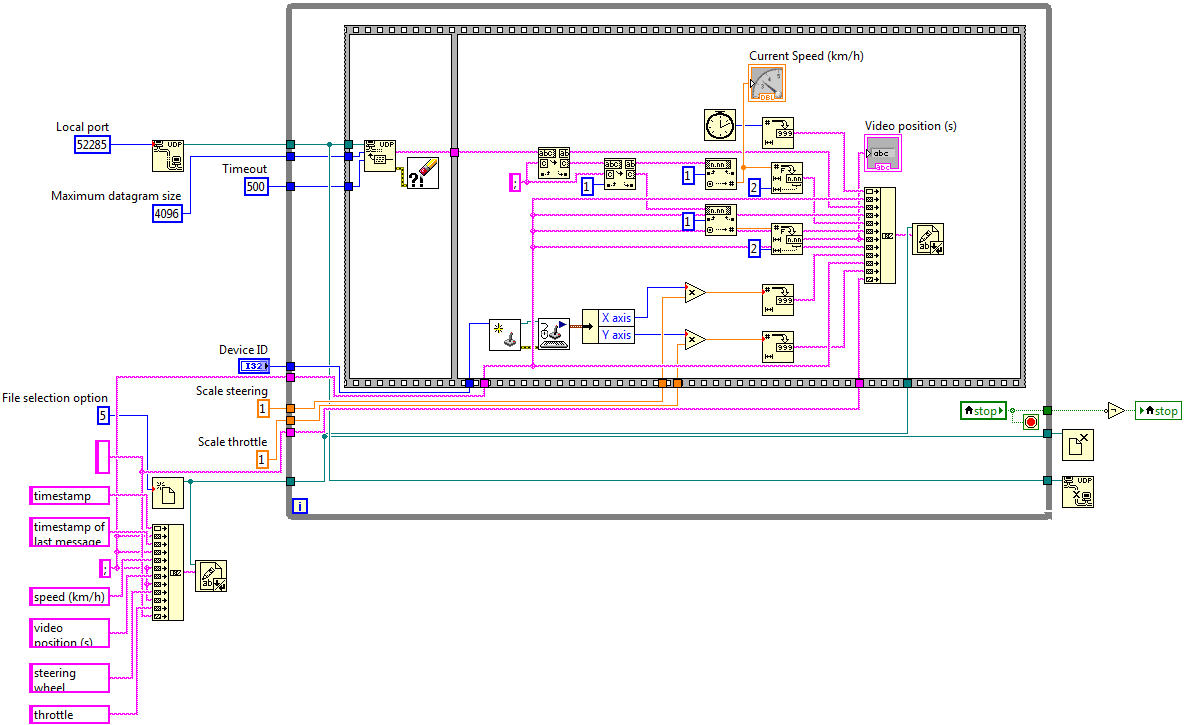
\includegraphics[angle=90,width=0.9\linewidth]{src/labview_screenshot_videoplayer_daten_empfangen.png}
\caption{LabVIEW: Daten empfangen} % Titel der Grafik
\label{labview_screenshot_videoplayer_daten_empfangen} % Labelname
\end{figure}

\newpage

\subsubsection{UDP-Listener}
Der UDP-Listener empfängt die Packete, die vom LabVIEW gesendet werden. Diese werden ausgepackt und die übermittelten Werte abgespeichert. Der UDP-Listener wird im Kapitel \ref{sec:udp-listener} genau dokumentiert. 
\subsubsection{Hauptprogramm}
Das Hauptprogramm startet den MPlayer und den UDP-Listener. Der MPlayer wird, um ein Video abzuspielen, in einem eigenen Prozess gestartet. Der MPlayer kann duch einen speziellen Aufruf von der Komandozeile, wie im Listing \ref{start_mplayer} beschrieben, im Slavemodus gestartet werden. Wie der mPlayer im Videoplayer aufgerufen wird, kann dem Quellcod auf der Beiliegenden CD entnommen werden. 
\begin{lstlisting}[caption={Starten des MPlayers in einem eigenen Prozess}, label={start_mplayer}]
mplayer.exe -slave -hardframedrop -osdlevel 0 BeispielVideo.mp4
\end{lstlisting}
Der Parameter \textit{hardframedrop} dient der erhöhung der Framerate. Es wird bei hohen Abspielgeschwindigkeiten nicht jedes Bild angezeigt, sondern beispielsweise nur jedes dritte. Der \textit{osdlevel} Parameter bestimmt wieviel Information auf dem Bildschrim angezeigt wird. Der Level null unterdrückt jegliche Ausgaben.\\
In diesem Slavemodus nimmt der mPlayer Befehle die über die Kommandozeile abgesetzt werden entgegen. Dazu wird der Standard Ausgabepipe der Komandozeile an den mPlayer umgeleitet. Dann können einfache Befehel wie im Listing \ref{mplayer_befehl} an den mPlayer gesendet werden um das Video schneller oder langsamer Abspielen zu lassen. 
\begin{lstlisting}[caption={Befehl an den mPlayer über den Stardard Ausgabe Pipe}, label={mplayer_befehl}]
"speed_set %lf\n", speed
\end{lstlisting}
Im Listing \ref{mplayer_befehl} quantifiziert \textit{speed} die Abspielgeschwindigkeit in der das Video abgespielt werden soll. 